% ---------------------------------------------
% Alle Abbildungen 'images/' in Latex speichern 
%     * 'archiv/Pics-files.tex' 
%     * Bildgröße: 0.80/1 
% ju 08-Okt-2020 Pics-files.tex
% ---------------------------------------------
%
%\section{Chili-1}
%
%Chili-1 (\autoref{fig:Chili-1}).% Referenz
%
\begin{figure}[!hb]% hier: !hb
    \centering
  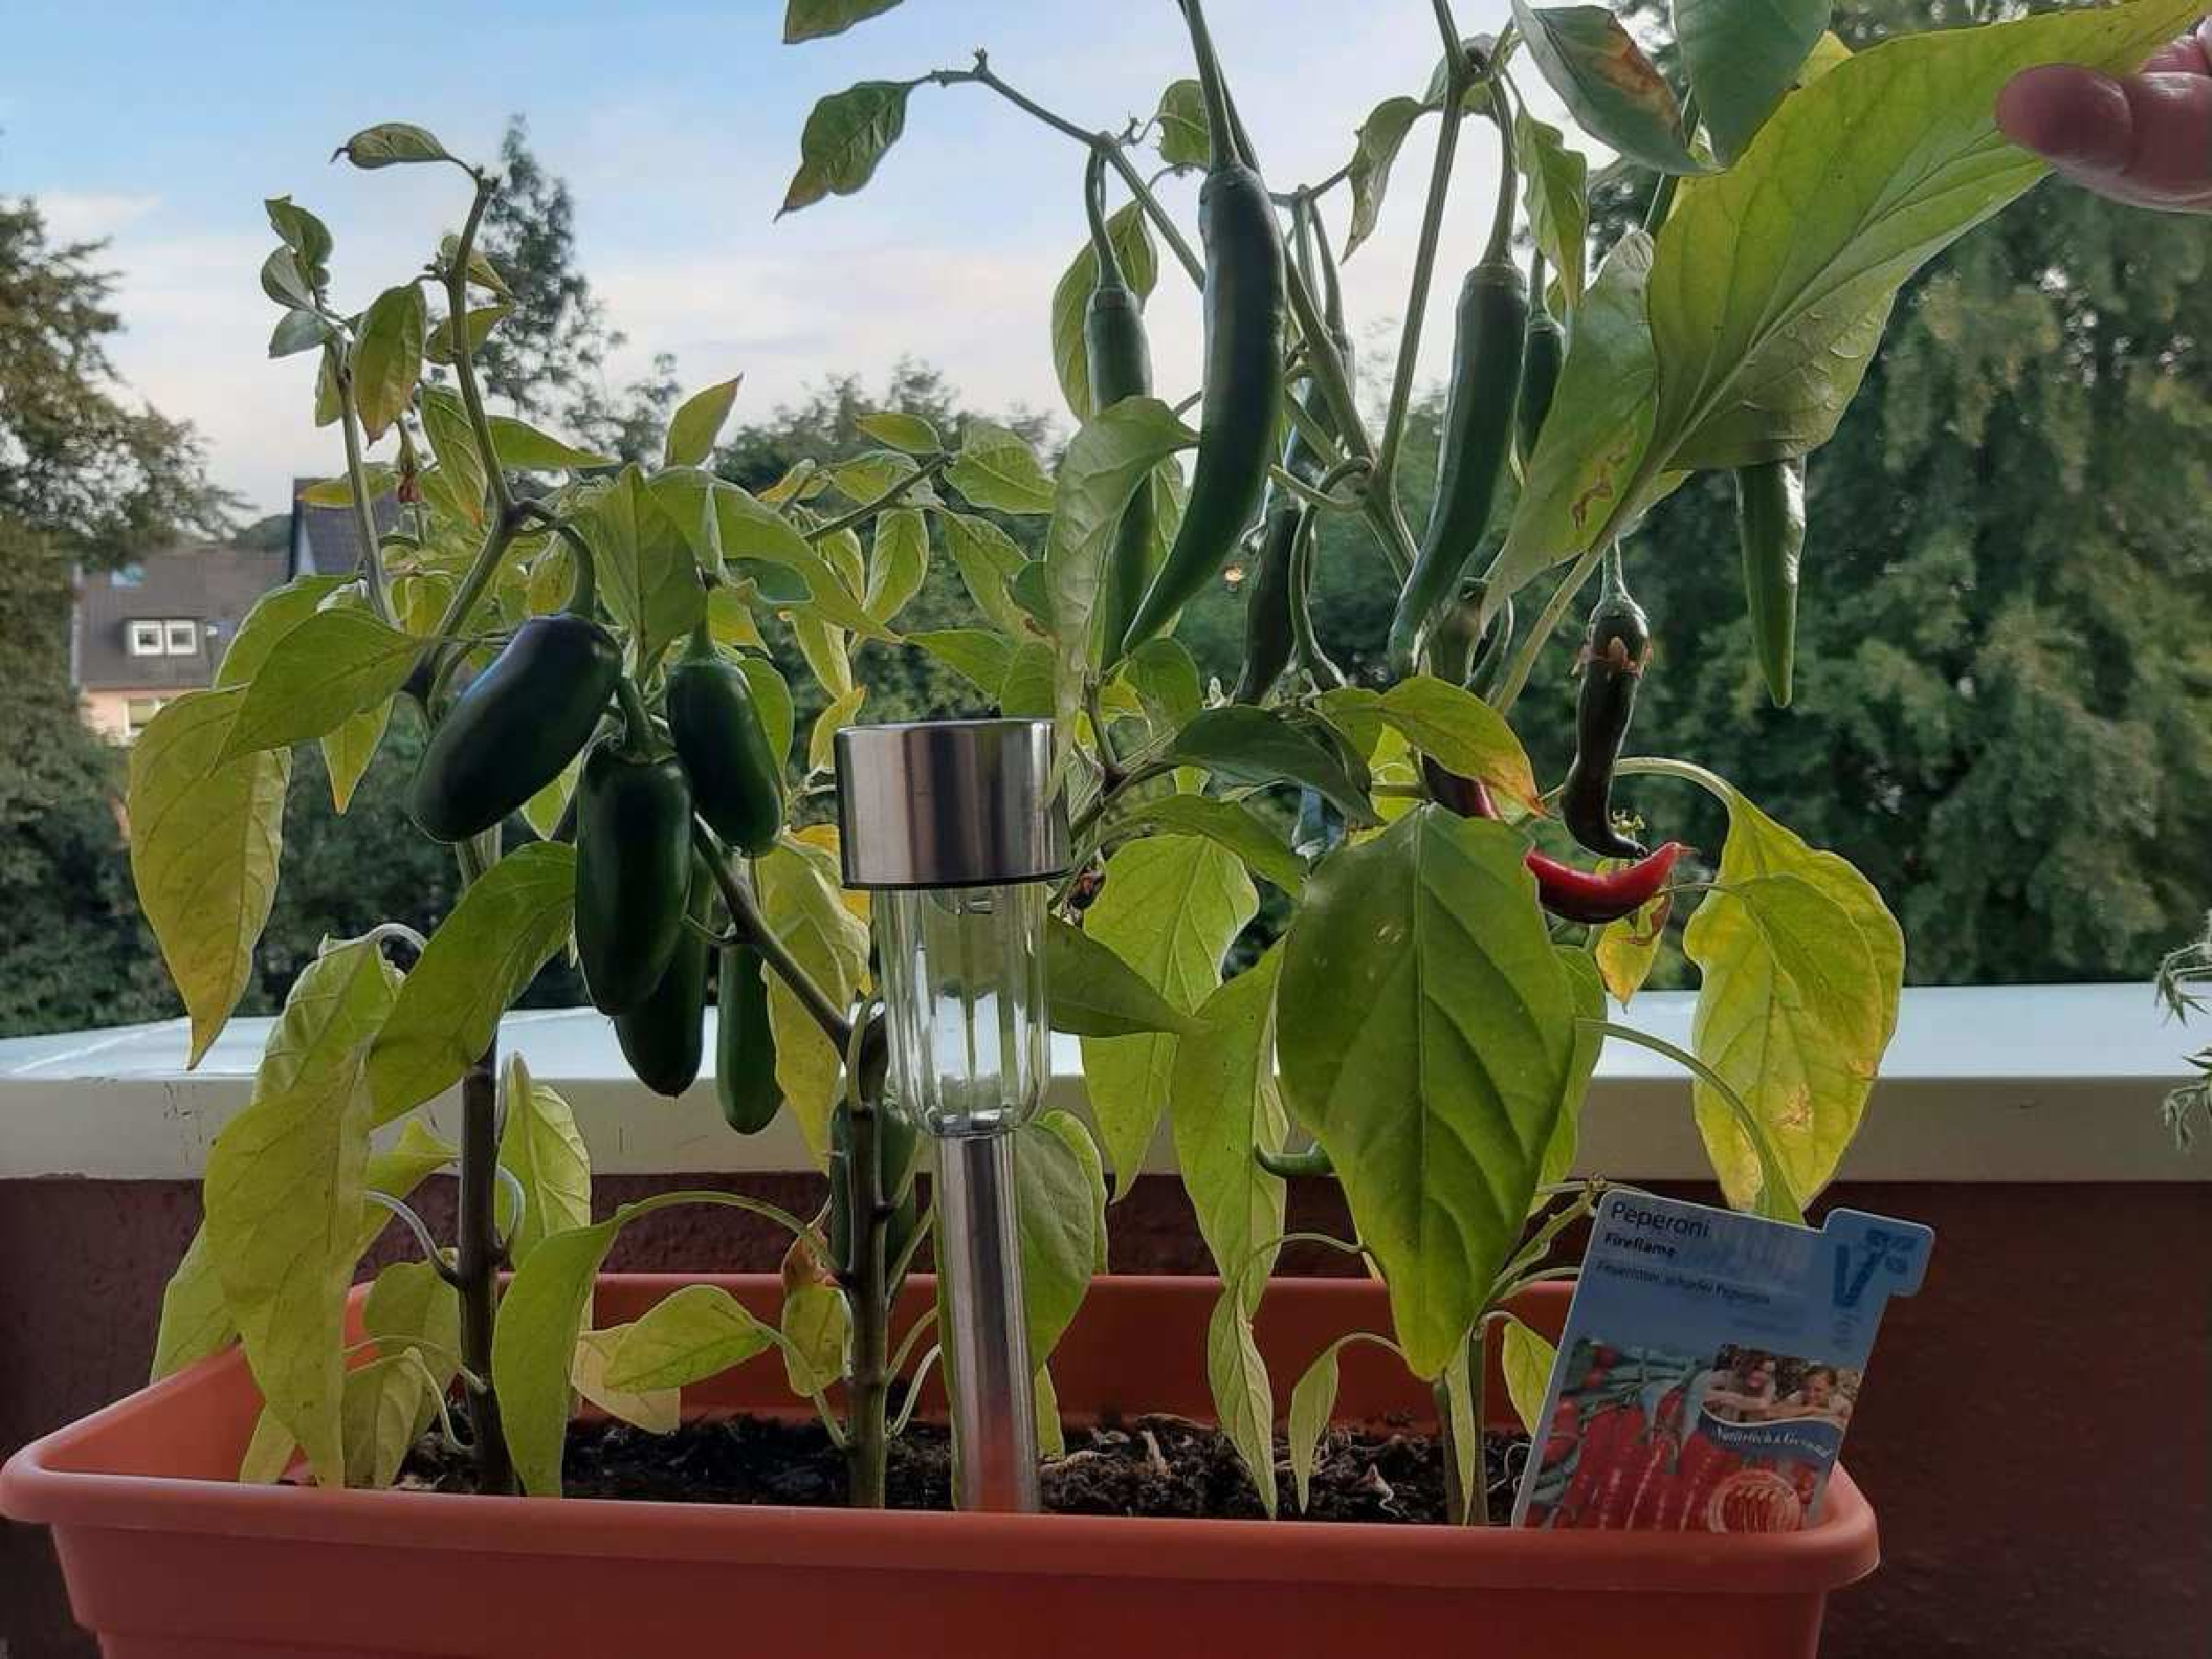
\includegraphics[width=.80\textwidth]{images/Chili-1.pdf}%
  \caption{Chili-1}%\label{fig:Chili-1}%% anpassen
\end{figure}

%\newpage
